\input{../documents-common/preamble.tex}
\usepackage{listings}             % Include the listings-package
\begin{document}
\maketitle[Finite Element Methods]{Assignment 1}

\section{introduction}
In this report we will discuss the effect on the error bounds of a finite element method
that changing the underlying mesh has, using the Poisson Equation:
\begin{align}
 -u'' = f,\; -1 < x < 1,\\
 u(-1) = u(1) = 0.
\end{align}
Here $u$ is the function of interest, and $f$ the driving force, which is taken to be equal to
\begin{align}
  f(x) = e^{-1000x^2}+10^{-3}
\end{align}
 Furthermore we will derive an a-posteriori error-bound on $\norm{u'}$.

\section{a-posteriori error-estimate}
Using the notation $\norm{\cdot}$ to indicate the $L^2$ norm over the whole domain and $\norm{\cdot}_i$ to indicate the $L^2$ norm over the interval $[x_{i-1}, x_i]$:
\begin{align}
 \norm{e'}^2 &= \sum^N_{i=1} \int_{x_{i-1}}^{x_i} e'(e-\pi e)'\d x\nn
 &= \sum^N_{i=1} \int_{x_{i-1}}^{x_i} (-e'')(e-\pi e)\d x + \left[e'(e-\pi e)\right]_{x_i -1}^{x_i}\nn
 &= \sum^N_{i=1} \int_{x_{i-1}}^{x_i} (-e'')(e-\pi e)\d x\nn
 &= \sum^N_{i=1} \int_{x_{i-1}}^{x_i} (-(u-u_h)'')(e-\pi e)\d x\nn
 &= \sum^N_{i=1} \int_{x_{i-1}}^{x_i} (f+u_h'')(e-\pi e)\d x\nn
 &\leq \sum^N_{i=1} \norm{f+u_h''}_i \norm{e-\pi e}_i\nn
 &\leq \sum^N_{i=1} h_i\norm{f+u_h''}_i C\norm{e'}_i\nn
 &\leq C\sqrt{\sum^N_{i=1} h_i^{\;2}\norm{f+u_h''}_i^{\;2}}\sqrt{\sum^N_{i=1} \norm{e'}_i^{\;2}}\nn
 &\leq C\sqrt{\sum^N_{i=1} \rho_i^{\;2}}\norm{e'}\nn
 \to \norm{e'} &\leq C\sqrt{\sum^N_{i=1} \rho_i^{\;2}}
\end{align}
\par It is known that in the 1D case the constant $C$ is unity.\footnote{{\em The Finite Element Method: Theory, Implementation, and Applications} page 7}

\section{The Finite Element Implementation}
We modeled the problem using a finite element method and the standard hat-functions, defined by
\begin{align}
 \phi_i(x_{i-1} \leq x \leq x_i) = (x-x_{i-1})/h,\nn
 \phi_i(x_{i} \leq x \leq x_{i+1}) = (x_{i+1}-x)/h,\nn
 \phi_i(x \setminus [x_{i-1}, x_{i+1}]) = 0.
\end{align}
\par The boundary conditions were enforced by replacing
the first and last row of the stiffness matrix $A$ by their respective unit-vectors
 and the first and last element of the load vector $b$ by the boundary values.
 \par After we have computed our initial solution, we compute the Laplacian by solving
 \begin{align}
   M\chi = -A \xi
 \end{align}
for $\chi$. Here $M$ is the mass matrix, defined by
\begin{align}
 M_{ij} = \int_0^1 \phi_j(x)\phi_i(x)\,\d x
\end{align}.
We subsequent compute $\rho_i$ using the trapezoidal rule for the interior points, that is:
\begin{align}
  \rho_i = \frac{1}{2}h_i^{\,2}\left((f(x_{i-1})+\chi_{i-1})+(f(x_i)+\chi_i)\right),
\end{align}
For the boundray intervals, we use a single pair of $\chi$ and $f$ instead.

\section{Adaptive Mesh Refinement}
Having obtained a set of $\rho_i$ (and thus an estimate of the error), we refine our mesh by subdividing each interval $i$ for which
\begin{align}
 \rho_i > \lambda \max_{i}(\rho_i),\;\lambda \in [0, 1].
\end{align}
We have tested $\lambda = 0.05, 0.25, 0.5, 1$, starting from 5 nodes and stopping once we have more than 1000 nodes.

\section{Results}
Our results are contained in figure \ref{fig:result}, \ref{fig:error}, and \ref{fig:spacing}.
\par Looking at figure \ref{fig:result} we note that the result becomes less smooth for increasing $\lambda$ near its inflection point, as the algorithm puts less points there for higher $\lambda$.
Visually, all results look similar.
\par Looking at the total error estimate in figure \ref{fig:error} we see that higher values of $\lambda$ perform better by up to two orders of magnitude for the same amount of points $N$. It should be note however, that for high values of $\lambda$ the mesh refinement algorithm takes significantlly longer to reach $N=1000$ as it adds fewer points per iteration.
\par Finally, figure \ref{fig:spacing} shows how the density of points changes with $\lambda$. Surprisingly, larger values of $\lambda$ give a more uniform distribution while $\lamba = 0$ will always give a perfectly uniform distribution.
\begin{figure}
\centering
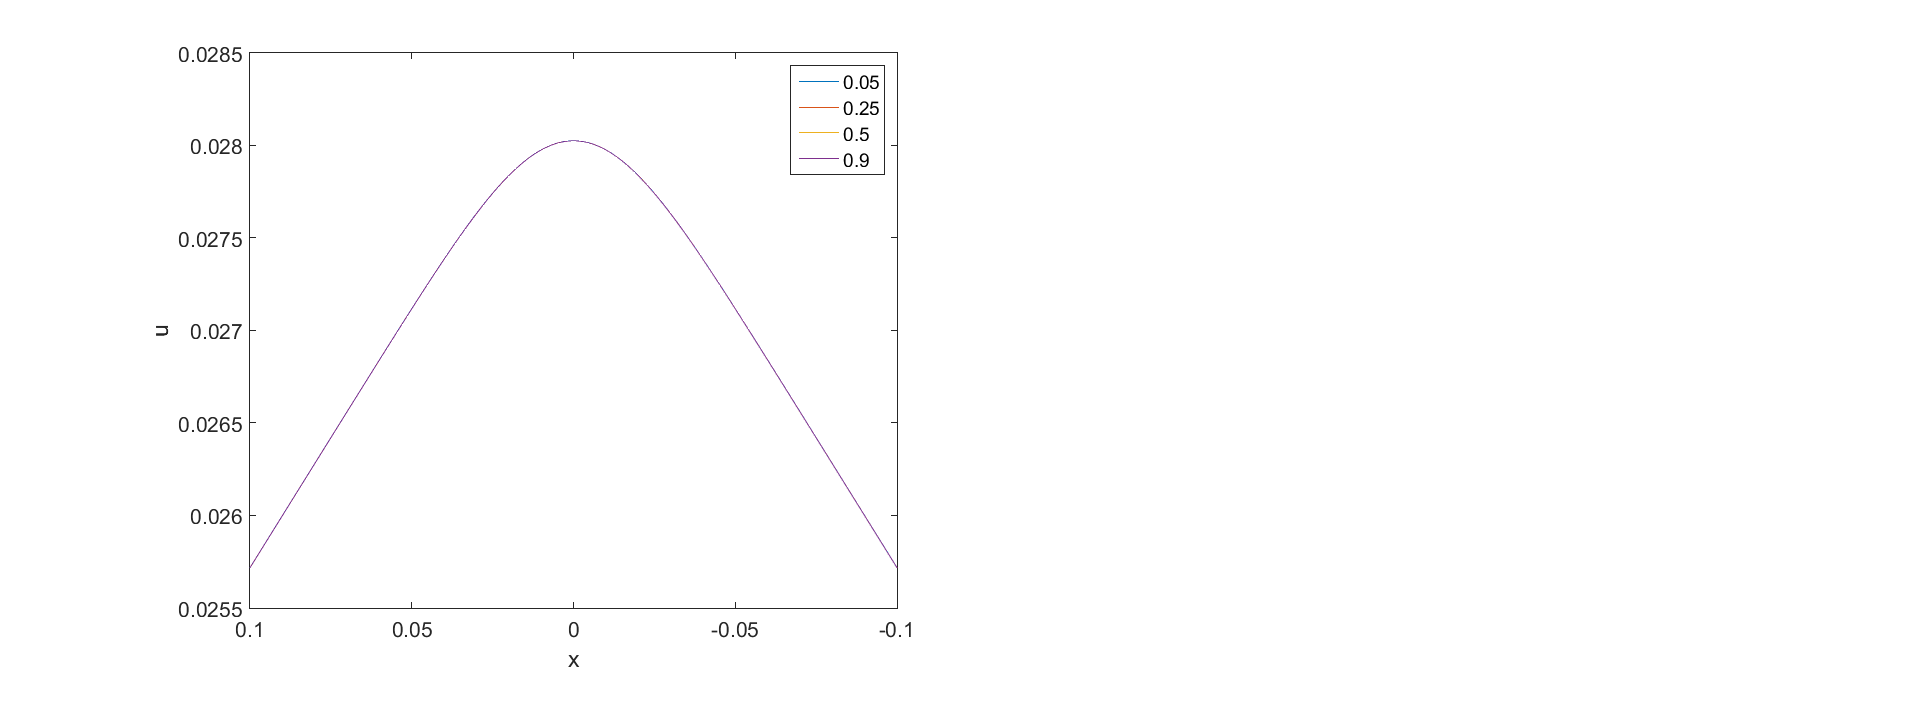
\includegraphics[width=2\textwidth]{figures/result}
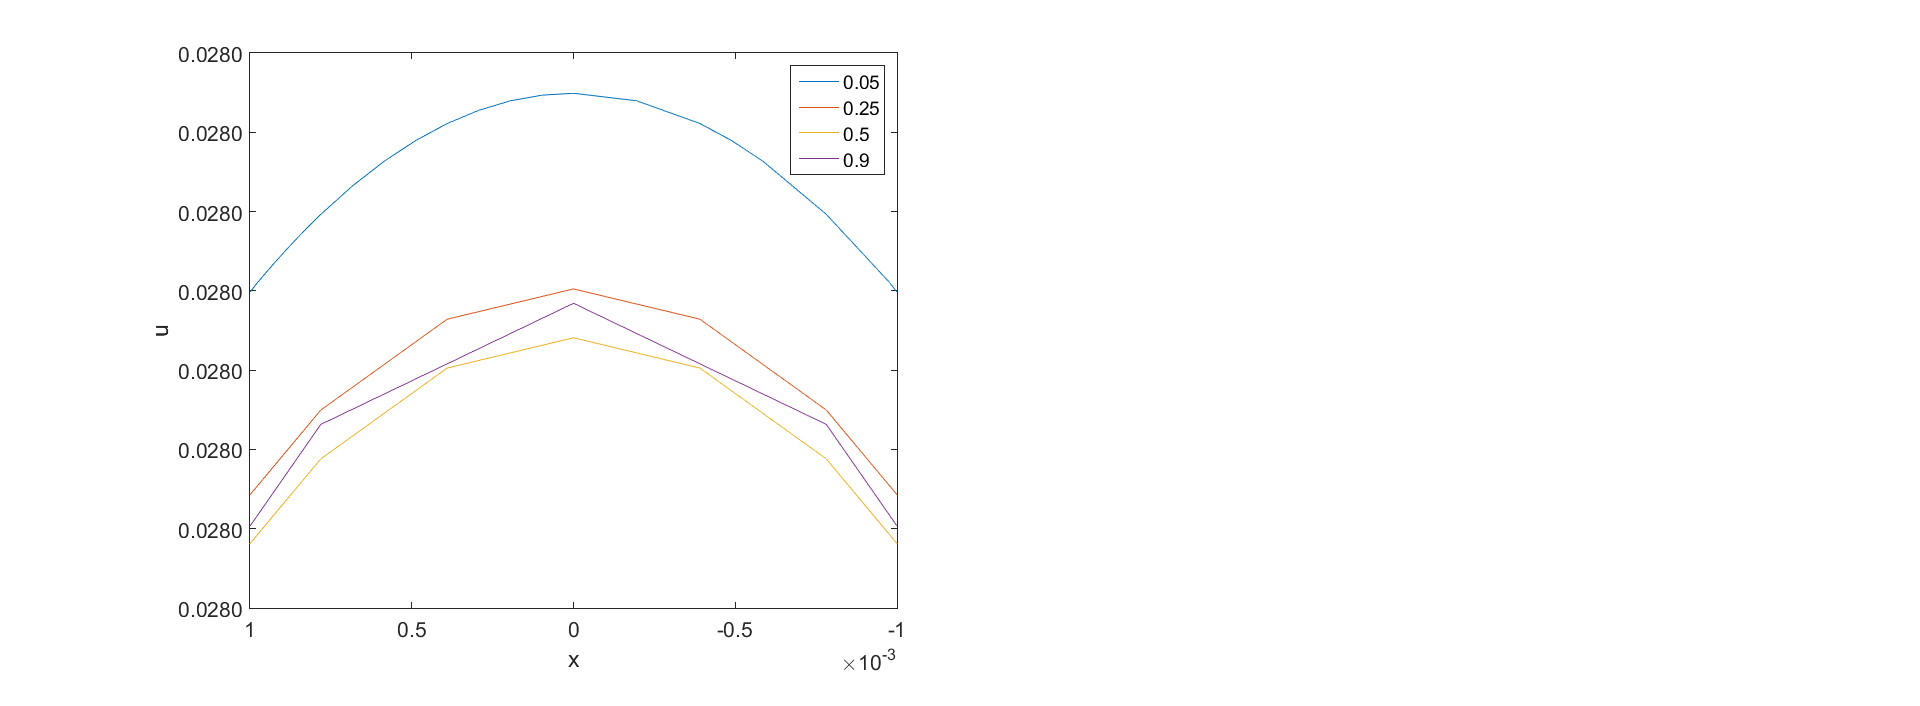
\includegraphics[width=2\textwidth]{figures/zoom}
\caption{The result of our method for different values of $\lambda$.}
\label{fig:result}
\end{figure}

\begin{figure}
\centering
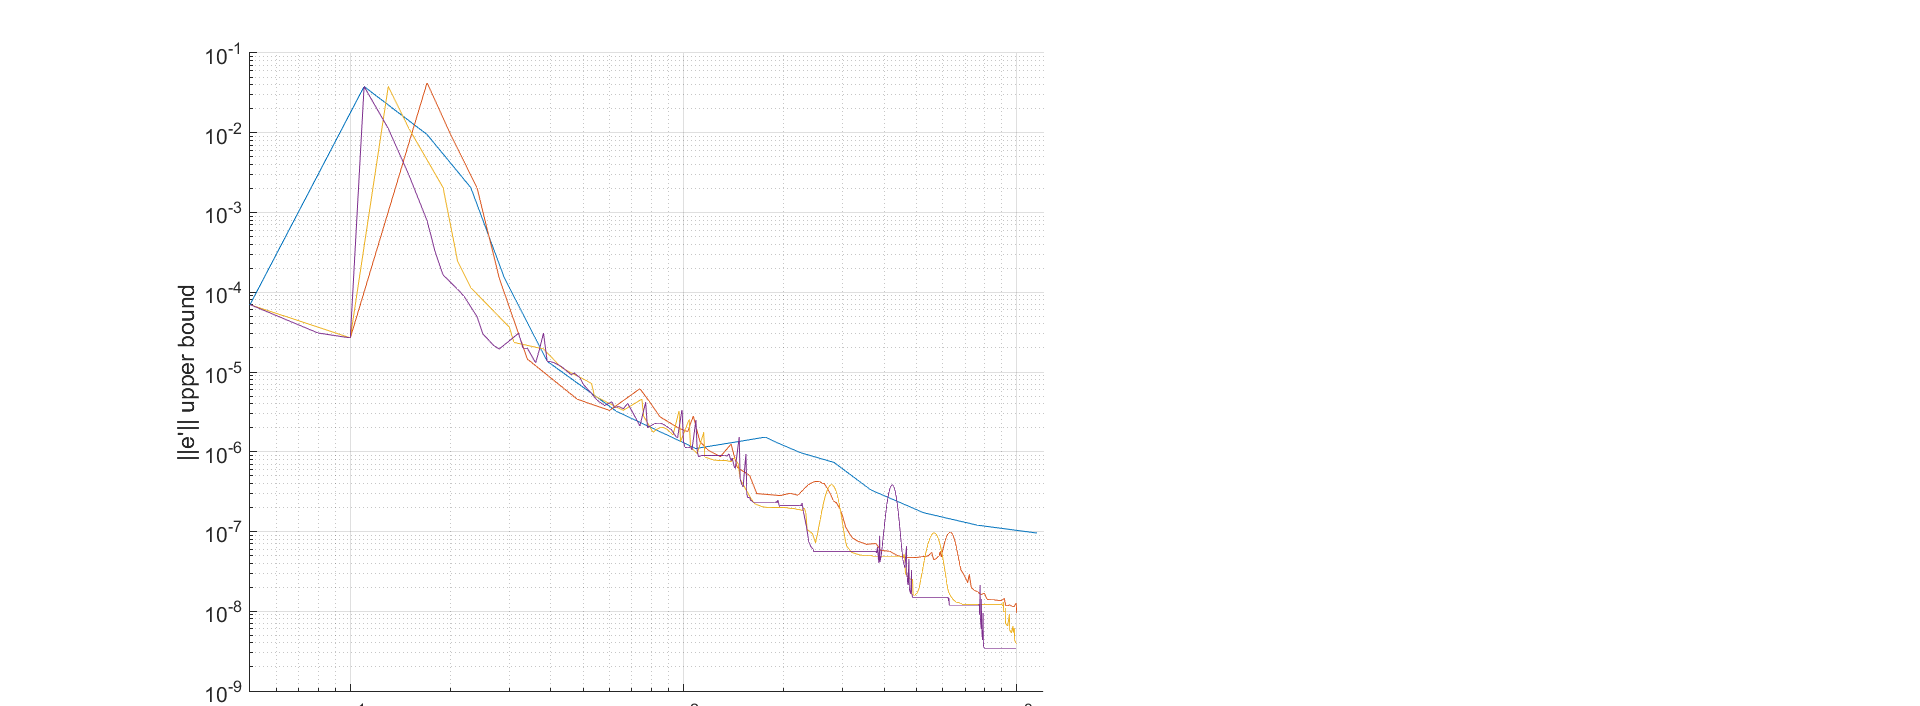
\includegraphics[width=1.5\textwidth]{figures/error}
\caption{The total sum of $\rho_i^{\,2}$ for different values of $\lambda$.}
\label{fig:error}
\end{figure}

\begin{figure}
\centering
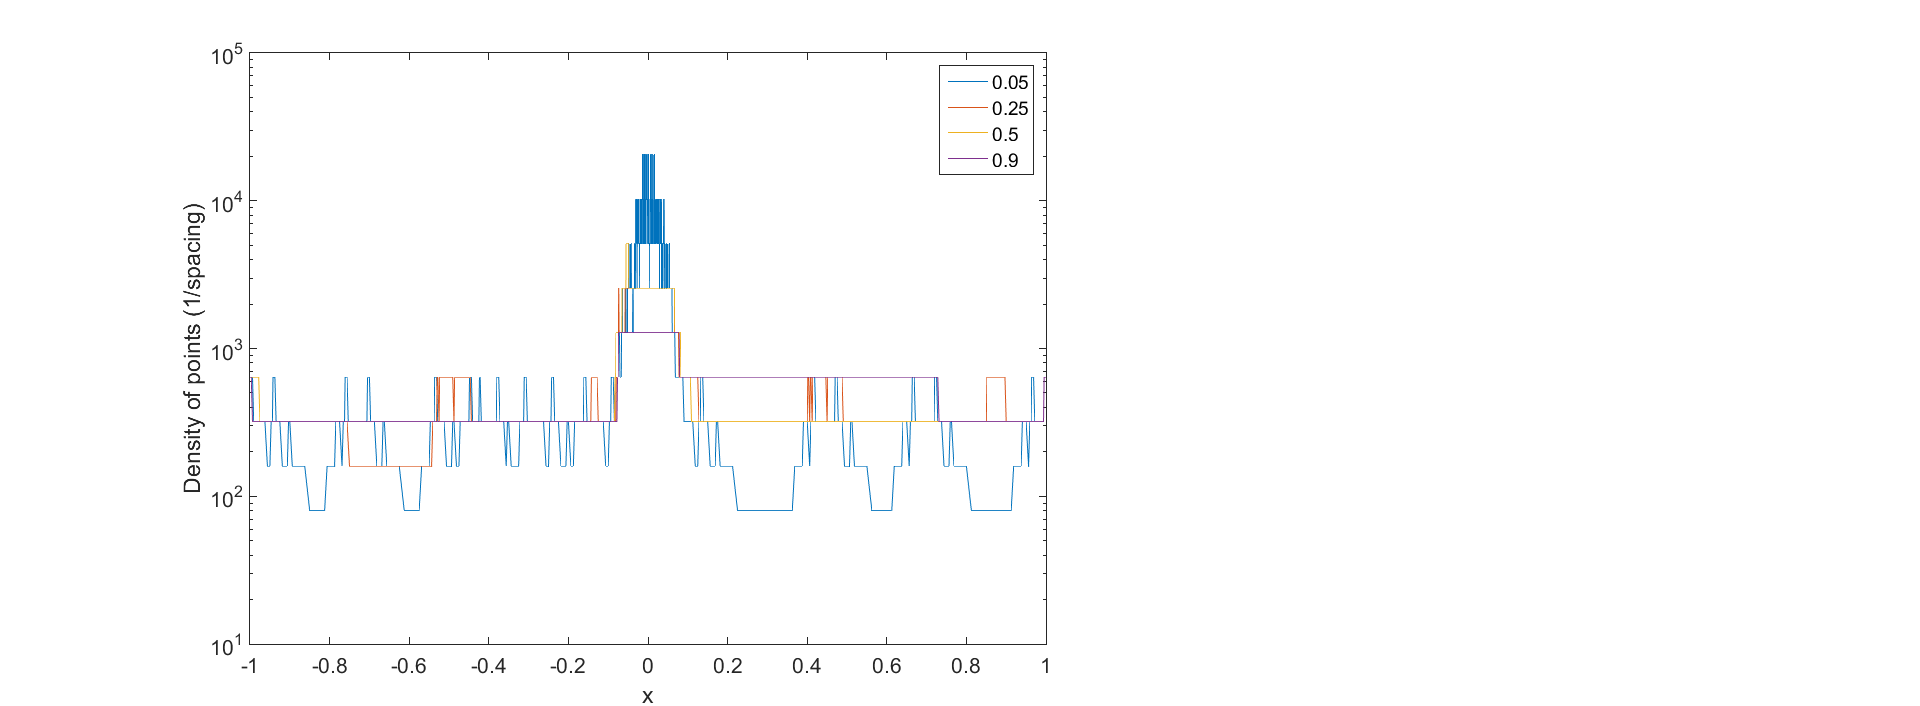
\includegraphics[width=1.5\textwidth]{figures/spacing}
\caption{The density of points for different values of $\lambda$.}
\label{fig:spacing}
\end{figure}
\newpage
\section{Code}
\subsection{Adaptive}
\lstinputlisting{./code/adaptive.m}
\subsection{Mass Matrix}
\lstinputlisting{./code/mass_matrix.m}
\subsection{Trapezoidal}
\lstinputlisting{./code/trapezoidal.m}


\end{document}
